%% LyX 2.3.6 created this file.  For more info, see http://www.lyx.org/.
%% Do not edit unless you really know what you are doing.
\documentclass[journal,article,submit,pdftex,moreauthors]{mdpi}
\usepackage[utf8]{inputenc}
\usepackage{float}
\usepackage{url}
\usepackage{graphicx}

\makeatletter

%%%%%%%%%%%%%%%%%%%%%%%%%%%%%% LyX specific LaTeX commands.

\Title{Training artificial neural networks using a global optimization method
that utilizes neural networks}

\TitleCitation{Training artificial neural networks using a global optimization method
that utilizes neural networks}

\Author{Ioannis G. Tsoulos$^{1,*}$, Alexandros Tzallas$^{2}$}

\AuthorNames{Ioannis G. Tsoulos, Alexandros Tzallas}

\AuthorCitation{Tsoulos, I.G.; Tzallas A.}


\address{$^{1}$\quad{}Department of Informatics and Telecommunications,
University of Ioannina, Greece\\
$^{2}\quad$Department of Informatics and Telecommunications, University
of Ioannina, Greece}


\corres{Correspondence: itsoulos@uoi.gr; }


\abstract{Perhaps one of the best-known machine learning models is that of
artificial neural networks, where a number of parameters must be adjusted
to learn a wide range of practical problems from areas such as Physics,
Chemistry, Medicine, etc. Such problems can be reduced to pattern
recognition problems and then modeled from artificial neural networks,
whether these problems are classification problems or regression problems.
To achieve the goal of neural networks, they must be trained by appropriately
adjusting their parameters using some global optimization methods.
In this work, the application of a recent global minimization technique
is suggested for the adjustment of neural network parameters. In this
technique, an approximation of the objective function to be minimized
is created using artificial neural networks and then sampling is done
from the approximation function and not the original one. Therefore,
in the present work, learning of the parameters of artificial neural
networks is done using other neural networks. The new training method
was tested on a series of well-known problems and a comparative study
was made against other neural network parameter tuning techniques
and the results were more than promising. From what was seen after
running the experiments and comparing the proposed technique with
others that have been used for classification datasets as well as
regression datasets, there was a significant difference in the performance
of the proposed technique, starting with 30\% for classification datasets
and reaching 50\% for regression problems. However, the proposed technique,
since it presupposes the use of global optimization techniques involving
artificial neural networks, may require significantly higher execution
time than other techniques.}


\keyword{Global optimization; Neural networks; Stochastic methods}

\DeclareTextSymbolDefault{\textquotedbl}{T1}
%% Because html converters don't know tabularnewline
\providecommand{\tabularnewline}{\\}

%%%%%%%%%%%%%%%%%%%%%%%%%%%%%% User specified LaTeX commands.
%  LaTeX support: latex@mdpi.com 
%  For support, please attach all files needed for compiling as well as the log file, and specify your operating system, LaTeX version, and LaTeX editor.

%=================================================================


% For posting an early version of this manuscript as a preprint, you may use "preprints" as the journal and change "submit" to "accept". The document class line would be, e.g., \documentclass[preprints,article,accept,moreauthors,pdftex]{mdpi}. This is especially recommended for submission to arXiv, where line numbers should be removed before posting. For preprints.org, the editorial staff will make this change immediately prior to posting.

%--------------------
% Class Options:
%--------------------
%----------
% journal
%----------
% Choose between the following MDPI journals:
% acoustics, actuators, addictions, admsci, adolescents, aerospace, agriculture, agriengineering, agronomy, ai, algorithms, allergies, alloys, analytica, animals, antibiotics, antibodies, antioxidants, applbiosci, appliedchem, appliedmath, applmech, applmicrobiol, applnano, applsci, aquacj, architecture, arts, asc, asi, astronomy, atmosphere, atoms, audiolres, automation, axioms, bacteria, batteries, bdcc, behavsci, beverages, biochem, bioengineering, biologics, biology, biomass, biomechanics, biomed, biomedicines, biomedinformatics, biomimetics, biomolecules, biophysica, biosensors, biotech, birds, bloods, blsf, brainsci, breath, buildings, businesses, cancers, carbon, cardiogenetics, catalysts, cells, ceramics, challenges, chemengineering, chemistry, chemosensors, chemproc, children, chips, cimb, civileng, cleantechnol, climate, clinpract, clockssleep, cmd, coasts, coatings, colloids, colorants, commodities, compounds, computation, computers, condensedmatter, conservation, constrmater, cosmetics, covid, crops, cryptography, crystals, csmf, ctn, curroncol, currophthalmol, cyber, dairy, data, dentistry, dermato, dermatopathology, designs, diabetology, diagnostics, dietetics, digital, disabilities, diseases, diversity, dna, drones, dynamics, earth, ebj, ecologies, econometrics, economies, education, ejihpe, electricity, electrochem, electronicmat, electronics, encyclopedia, endocrines, energies, eng, engproc, ent, entomology, entropy, environments, environsciproc, epidemiologia, epigenomes, est, fermentation, fibers, fintech, fire, fishes, fluids, foods, forecasting, forensicsci, forests, foundations, fractalfract, fuels, futureinternet, futureparasites, futurepharmacol, futurephys, futuretransp, galaxies, games, gases, gastroent, gastrointestdisord, gels, genealogy, genes, geographies, geohazards, geomatics, geosciences, geotechnics, geriatrics, hazardousmatters, healthcare, hearts, hemato, heritage, highthroughput, histories, horticulturae, humanities, humans, hydrobiology, hydrogen, hydrology, hygiene, idr, ijerph, ijfs, ijgi, ijms, ijns, ijtm, ijtpp, immuno, informatics, information, infrastructures, inorganics, insects, instruments, inventions, iot, j, jal, jcdd, jcm, jcp, jcs, jdb, jeta, jfb, jfmk, jimaging, jintelligence, jlpea, jmmp, jmp, jmse, jne, jnt, jof, joitmc, jor, journalmedia, jox, jpm, jrfm, jsan, jtaer, jzbg, kidney, kidneydial, knowledge, land, languages, laws, life, liquids, literature, livers, logics, logistics, lubricants, lymphatics, machines, macromol, magnetism, magnetochemistry, make, marinedrugs, materials, materproc, mathematics, mca, measurements, medicina, medicines, medsci, membranes, merits, metabolites, metals, meteorology, methane, metrology, micro, microarrays, microbiolres, micromachines, microorganisms, microplastics, minerals, mining, modelling, molbank, molecules, mps, msf, mti, muscles, nanoenergyadv, nanomanufacturing, nanomaterials, ncrna, network, neuroglia, neurolint, neurosci, nitrogen, notspecified, nri, nursrep, nutraceuticals, nutrients, obesities, oceans, ohbm, onco, oncopathology, optics, oral, organics, organoids, osteology, oxygen, parasites, parasitologia, particles, pathogens, pathophysiology, pediatrrep, pharmaceuticals, pharmaceutics, pharmacoepidemiology, pharmacy, philosophies, photochem, photonics, phycology, physchem, physics, physiologia, plants, plasma, pollutants, polymers, polysaccharides, poultry, powders, preprints, proceedings, processes, prosthesis, proteomes, psf, psych, psychiatryint, psychoactives, publications, quantumrep, quaternary, qubs, radiation, reactions, recycling, regeneration, religions, remotesensing, reports, reprodmed, resources, rheumato, risks, robotics, ruminants, safety, sci, scipharm, seeds, sensors, separations, sexes, signals, sinusitis, skins, smartcities, sna, societies, socsci, software, soilsystems, solar, solids, sports, standards, stats, stresses, surfaces, surgeries, suschem, sustainability, symmetry, synbio, systems, taxonomy, technologies, telecom, test, textiles, thalassrep, thermo, tomography, tourismhosp, toxics, toxins, transplantology, transportation, traumacare, traumas, tropicalmed, universe, urbansci, uro, vaccines, vehicles, venereology, vetsci, vibration, viruses, vision, waste, water, wem, wevj, wind, women, world, youth, zoonoticdis 

%---------
% article
%---------
% The default type of manuscript is "article", but can be replaced by: 
% abstract, addendum, article, book, bookreview, briefreport, casereport, comment, commentary, communication, conferenceproceedings, correction, conferencereport, entry, expressionofconcern, extendedabstract, datadescriptor, editorial, essay, erratum, hypothesis, interestingimage, obituary, opinion, projectreport, reply, retraction, review, perspective, protocol, shortnote, studyprotocol, systematicreview, supfile, technicalnote, viewpoint, guidelines, registeredreport, tutorial
% supfile = supplementary materials

%----------
% submit
%----------
% The class option "submit" will be changed to "accept" by the Editorial Office when the paper is accepted. This will only make changes to the frontpage (e.g., the logo of the journal will get visible), the headings, and the copyright information. Also, line numbering will be removed. Journal info and pagination for accepted papers will also be assigned by the Editorial Office.

%------------------
% moreauthors
%------------------
% If there is only one author the class option oneauthor should be used. Otherwise use the class option moreauthors.

%---------
% pdftex
%---------
% The option pdftex is for use with pdfLaTeX. If eps figures are used, remove the option pdftex and use LaTeX and dvi2pdf.

%=================================================================
% MDPI internal commands
\firstpage{1} 
 
\setcounter{page}{\@firstpage} 

\pubvolume{1}
\issuenum{1}
\articlenumber{0}
\pubyear{2022}
\copyrightyear{2022}
%\externaleditor{Academic Editor: Firstname Lastname} % For journal Automation, please change Academic Editor to "Communicated by"
\datereceived{} 
\dateaccepted{} 
\datepublished{} 
%\datecorrected{} % Corrected papers include a "Corrected: XXX" date in the original paper.
%\dateretracted{} % Corrected papers include a "Retracted: XXX" date in the original paper.
\hreflink{https://doi.org/} % If needed use \linebreak
%\doinum{}
%------------------------------------------------------------------
% The following line should be uncommented if the LaTeX file is uploaded to arXiv.org
%\pdfoutput=1

%=================================================================
% Add packages and commands here. The following packages are loaded in our class file: fontenc, inputenc, calc, indentfirst, fancyhdr, graphicx, epstopdf, lastpage, ifthen, lineno, float, amsmath, setspace, enumitem, mathpazo, booktabs, titlesec, etoolbox, tabto, xcolor, soul, multirow, microtype, tikz, totcount, changepage, attrib, upgreek, cleveref, amsthm, hyphenat, natbib, hyperref, footmisc, url, geometry, newfloat, caption

%=================================================================
%% Please use the following mathematics environments: Theorem, Lemma, Corollary, Proposition, Characterization, Property, Problem, Example, ExamplesandDefinitions, Hypothesis, Remark, Definition, Notation, Assumption
%% For proofs, please use the proof environment (the amsthm package is loaded by the MDPI class).

%=================================================================
% The fields PACS, MSC, and JEL may be left empty or commented out if not applicable
%\PACS{J0101}
%\MSC{}
%\JEL{}

%%%%%%%%%%%%%%%%%%%%%%%%%%%%%%%%%%%%%%%%%%
% Only for the journal Diversity
%\LSID{\url{http://}}

%%%%%%%%%%%%%%%%%%%%%%%%%%%%%%%%%%%%%%%%%%
% Only for the journal Applied Sciences:
%\featuredapplication{Authors are encouraged to provide a concise description of the specific application or a potential application of the work. This section is not mandatory.}
%%%%%%%%%%%%%%%%%%%%%%%%%%%%%%%%%%%%%%%%%%

%%%%%%%%%%%%%%%%%%%%%%%%%%%%%%%%%%%%%%%%%%
% Only for the journal Data:
%\dataset{DOI number or link to the deposited data set in cases where the data set is published or set to be published separately. If the data set is submitted and will be published as a supplement to this paper in the journal Data, this field will be filled by the editors of the journal. In this case, please make sure to submit the data set as a supplement when entering your manuscript into our manuscript editorial system.}

%\datasetlicense{license under which the data set is made available (CC0, CC-BY, CC-BY-SA, CC-BY-NC, etc.)}

%%%%%%%%%%%%%%%%%%%%%%%%%%%%%%%%%%%%%%%%%%
% Only for the journal Toxins
%\keycontribution{The breakthroughs or highlights of the manuscript. Authors can write one or two sentences to describe the most important part of the paper.}

%%%%%%%%%%%%%%%%%%%%%%%%%%%%%%%%%%%%%%%%%%
% Only for the journal Encyclopedia
%\encyclopediadef{Instead of the abstract}
%\entrylink{The Link to this entry published on the encyclopedia platform.}
%%%%%%%%%%%%%%%%%%%%%%%%%%%%%%%%%%%%%%%%%%

\makeatother

\begin{document}
\maketitle

\section{Introduction}

Artificial Neural Networks (ANNs) are parametric models \citep{nn1,nn2,nnreview}
that appeared in machine learning and they are widely used in pattern
recognition problems. A series of practical problems from the fields
of physics \citep{nnphysics1,nnphysics2,nnphysics3}, chemistry \citep{nnchem1,nnchem2,nnchem3},
economics \citep{nnecon1,nnecon2,nncecon3}, medicine \citep{nnmed1,nnmed2}
etc. can be transformed to pattern recognition problems and then solved
using Artificial Neural Networks.\textbf{ }Also, neural networks have
been used with success to solve differential equations \citep{nnde1,nnde2,nnde3},
solar radiation prediction \citep{nnsolar1,nnsolar2}, Spam detection
\citep{nnspam1,nnspam2,nnspam3} etc. Moreover, variations of artificial
neural networks have been employed to solve agricultural problems
\citep{nnagr1,nnagr2}, facial expression recognition \citep{nnfacial},
prediction of the speed of wind \citep{nnwind}, the gas consumption
problem \citep{nngas}, intrusion detection \citep{nnintrusion},
hydrological systems \citep{nnhydro1} etc. Also, Swales and Yoon
discuss the application of artificial neural networks to investment
analysis in their work \citep{nninvest}.

A neural network can be denoted as a function \textbf{$N(\overrightarrow{x},\overrightarrow{w})$
}where the vector $\overrightarrow{x}$ stands for the input vector
and the vector \textbf{$\overrightarrow{w}$ }is the set of the parameters
of the neural network that should be estimated. The input vector is
usually called pattern in the relevant literature and the vector \textbf{$\overrightarrow{w}$
}is usually called the weight vector. Artificial neural network training
methods adjust the vector of weights in order to minimize the following
quantity:
\begin{equation}
E\left(N\left(\overrightarrow{x},\overrightarrow{w}\right)\right)=\sum_{i=1}^{M}\left(N\left(\overrightarrow{x}_{i},\overrightarrow{w}\right)-y_{i}\right)^{2}\label{eq:eq1}
\end{equation}
In the previous equation, that will be called training error, the
set $\left(\overrightarrow{x_{i}},y_{i}\right),\ i=1,...,M$ is the
input train dataset for the neural network with $M$ patterns. The
value $y_{i}$ is the expected output for the pattern $\overrightarrow{x_{i}}$
. The Equation \ref{eq:eq1} can be minimized with respect to the
weight vector using any local or global optimization method like the
Back Propagation method \citep{bpnn,bpnn2}, the Hill Climbing method
\citep{nnhill}, the RPROP method \citep{rpropnn,rpropnn3,rpropnn2},
Quasi Newton methods \citep{quasinn,quasinn2}, Simulated Annealing
\citep{nn_ann1,nn_ann2}, Genetic Algorithms \citep{geneticnn,geneticnn2},
Particle Swarm Optimization \citep{psonn,psonn2},Differential Optimization
methods \citep{nndem,nndem2}, Evolutionary Computation \citep{nnevo},
the Whale optimization algorithm \citep{nnwhale} etc. Furthermore,
Cui et al suggested the usage of a new stochastic optimization algorithm
that simulates the plant growing process for neural network training.
Also recently, the Bird Mating Optimizer \citep{nnbird} was suggested
as a training method for artificial neural networks \citep{nnplant}.
Also, hybrid methods have been developed by various researchers to
optimize the weight vector, such as the work of Yaghini et al \citep{nnhybrid1}
that combined particle swarm optimization with a back propagation
algorithm to minimize the error function. Moreover, Chen at al \citep{nnhybrid2}
has used a hybrid technique that combines particle swarm optimization
and Cuckoo Search \citep{csmethod} to optimize the weight vector
of neural networks. 

In addition, many researchers have addressed the issue of initial
values for the weights of neural networks, such as the incorporation
of decision trees \citep{nninit1}, an initialization method using
the Cauchy's inequality \citep{weight_init2}, incorporation of discriminant
learning \citep{weight_init3}, methods based on genetic algorithms
\citep{nninit2,nninit3} etc. A paper discussing all the aspects of
weight initialization strategies can be found is proposed by Narkhede
et al \citep{nninitreview}.

Moreover, various groups of researchers are dealing with the issue
of constructing the structure of artificial neural networks, such
as the incorporation of genetic algorithms \citep{nngencon}, the
usage of the Grammatical Evolution method \citep{mainGe} for the
construction of neural networks\citep{nnc},\textbf{ }a constructing
and pruning approach to optimize the structure of ANNs \citep{nnprunncon},
usage of cellular automata\textbf{ }\citep{nncell} etc. Also, since
the training of artificial neural networks by optimization methods
requires significantly longer computing time, parallel techniques
have been developed that take advantage of modern parallel computing
units\citep{weight_gpu1,weight_gpu2,weight_gpu3}\textbf{.}

Another field of research in the field of artificial neural networks
that attracts a multitude of researchers is that of dealing with the
problem of overfitting that occurs in many cases. In this problem,
although the artificial neural network has achieved a satisfactory
level of training, this is not reflected in unknown patterns that
were not present during training. This set of patterns will be called
test set in the remaining of this work. Commonly used methods that
tackle the overfitting problem are weight sharing \citep{nnsharing1,nnsharing2},
methods that reduce the number of parameters (weight pruning) \citep{nnprunning1,nnprunning2,nnprunning3},
the method of dropout \citep{nndrop1,nndrop2}, weight decaying methods
\citep{nndecay1,nndecay2}, the Sarprop method \citep{sarprop}, positive
correlation methods \citep{nnpositive} etc. 

In this paper, the use of a recent global minimization technique \citep{nmin}
called NeuralMinimizer, is proposed to find the optimal set for the
weights of artificial neural networks. This innovative global minimization
technique constructs an approximation of the objective function to
be minimized using a limited number of its samples. These limited
samples form the training set of an artificial neural network that
can be trained with any optimization method. Subsequently, the sampling
for the continuation of the global optimization method is not done
by the objective function but by the already trained artificial neural
network. The samples obtained by artificial neural networks before
being fed into the global minimization method are classified and those
with the smallest functional value will finally be input into the
global minimization method. From the experimental results, it was
shown that this global minimization method requires a limited number
of samples from the objective function to find the global minimum
and is also more efficient than other techniques to discover the global
minimum. Therefore, this paper proposes using artificial neural networks
to train other artificial neural networks. This new procedure will
be tested on a series of known problems, in order to evaluate its
effectiveness.

The rest of this article is organized as follows: the section \ref{sec:The-proposed-method}
described the proposed method, the section \ref{sec:Experiments}
list the experimental datasets and the results obtained by the incorporation
of various methods and finally the section \ref{sec:Conclusions}
discusses some conclusions.

\section{The proposed method\label{sec:The-proposed-method}}

In this section, some basic principles for artificial neural networks
are presented and then a new training method that incorporates a modified
version of the NeuralMinimizer global optimization technique is outlined.

\subsection{Preliminaries}

Let us consider that we have an artificial neural network with just
one hidden layer, in which the sigmoid function is used as an activation
function. The output value for every node in this layer is calculated
as:
\begin{equation}
o_{i}(x)=\sigma\left(p_{i}x+\theta_{i}\right),\label{eq:eq1-1}
\end{equation}
where the value $p_{i}$ is the weight vector and $\theta_{i}$ denotes
the bias for the node $i.$ The sigmoid function is defined as:
\begin{equation}
\sigma(x)=\frac{1}{1+\exp\left(-x\right)}
\end{equation}
 and it is graphically illustrated in Figure \ref{fig:sigx}.

\begin{figure}[H]
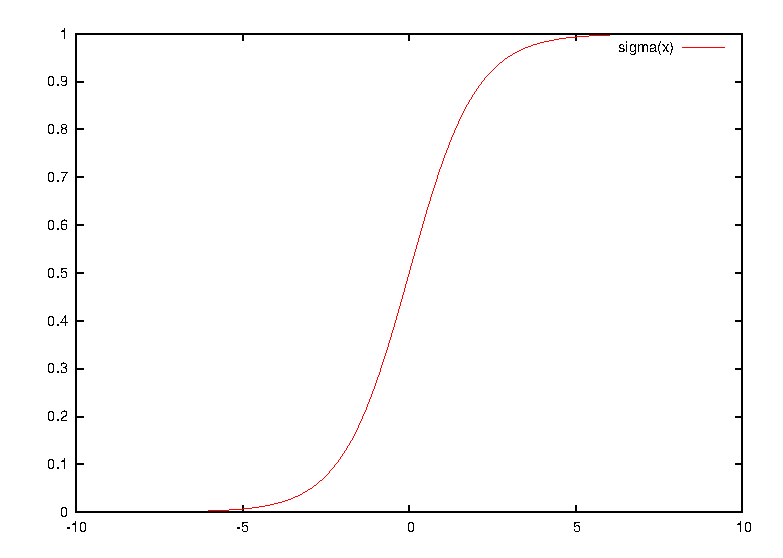
\includegraphics[scale=0.7]{sig}

\caption{The sigmoid function $\sigma(x)$.\label{fig:sigx}}

\end{figure}
When the neural network has $H$ processing nodes, then output can
be formulated as:
\begin{equation}
N(x)=\sum_{i=1}^{H}v_{i}o_{i}(x),\label{eq:eq1-2}
\end{equation}
where $v_{i}$ stands for the output weight for node $i$. Hence,
by using one vector for all the parameters (weights and biases) the
neural network can be written in the following form:
\begin{equation}
N\left(\overrightarrow{x},\overrightarrow{w}\right)=\sum_{i=1}^{H}w_{(d+2)i-(d+1)}\sigma\left(\sum_{j=1}^{d}x_{j}w_{(d+2)i-(d+1)+j}+w_{(d+2)i}\right)\label{eq:nn}
\end{equation}
where $d$ is the dimension of vector $\overrightarrow{x}$. From
the Equation \ref{eq:nn} we can conclude that number of elements
in the weight vector have as:
\begin{equation}
d_{w}=(d+2)H\label{eq:wdimension}
\end{equation}


\subsection{The modified NeuralMinimizer method }

In its original version, the method NeuralMinimizer employed RBF neural
networks \citep{rbf1} to build a model of the objective function.
Even though Radial Basis Function (RBF) networks have been used with
success in a variety of problems \citep{rbfde1,rbfde2,rbfnetwork1,rbfnetwork2},
it is not possible to apply them to the training of the parameters
of an artificial neural network due to the large dimension of the
problem, as shown in Equation \ref{eq:wdimension}. Hence, in current
work, the RBF network has been replaced by an artificial neural network
that implements the Equation \ref{eq:nn}. The training of the artificial
neural network was done using a local minimization technique that
is not particularly demanding in calculations and storage space, such
as Limited Memory BFGS (L-BFGS)\citep{LBFGS}. Obviously, any other
technique that is not extremely memory intensive could be used in
its place. Such a technique could be the Adam method \citep{Adam},
the SGD method \citep{sgd1,sgd2} or even a simple global minimization
method such as a genetic algorithm with a limited number of chromosomes.
The L-BFGS method is a variation of the Broyden--Fletcher--Goldfarb--Shanno
(BFGS) method \citep{bfgs2} using a limited amount of computer memory.
This local minimization method has found wide application in difficult
and memory-intensive optimization problems such as image reconstruction
\citep{lbfgs_image}, inverse eigenvalue problems \citep{lbfgs_inverse},
seismic waveform tomography \citep{lbfgs_seismic} etc. Because of
the application of this technique to large-dimensional problems, a
number of modifications have been proposed that make use of modern
parallel computing systems \citep{lbfgs_par1,lbfgs_par2,lbfgs_par3}.
A numerical study on the limited memory BFGS methods is provided in
the work of Morales \citep{lbfgs_study}. In the original publication
of the NeuralMinimizer optimization method, an RBF neural network
was used to generate the approximation function of the objective function.
However, this would not always be possible in the case where the objective
function to be minimized is the error of an artificial neural network,
since an artificial neural network usually has a large number of parameters
and this would require an extremely large storage space for training
the global minimization method's RBF neural network.

In the following the main steps of the modified NeuralMinimizer method
for the training of neural networks are listed. In this steps the
neural network used by the NeuralMinimizer method will be called $N_{N}(x,w)$.
\begin{enumerate}
\item \textbf{Initialization} step.
\begin{enumerate}
\item \textbf{Set $H$ }the number of weights of the neural network. In
the current method the same number of weights was used for both $N(x,w)$
and $N_{N}(x,w)$ artificial neural networks.
\item \textbf{Set} $N_{S}$ as the samples that will be initially drawn
from $N(x,w)$. At this stage, the training error for the artificial
neural network will be used as an objective function to minimize
\item \textbf{Set} $N_{T}$ as the the number of points that will be utilized
as local minimization method starters in every iteration. 
\item \textbf{Set} $N_{R}$ the number of samples that will be drawn from
the $N_{N}(x,w)$ network in each iteration. 
\item \textbf{Set} $N_{G}$ as the maximum number of iterations allowed.
\item \textbf{Set} Iter=0, the current iteration number.
\item \textbf{Set} $\left(w^{*},y^{*}\right)$ as the global minimum discovered
by the method. Initially $y^{*}=\infty,\ w^{*}=\left(0,0,\ldots,0\right)$
\end{enumerate}
\item \textbf{Creation }Step.
\begin{enumerate}
\item \textbf{Set} $T=\emptyset$, the used training set for the $N_{N}(x,w)$
neural network.
\item \textbf{For} $i=1,..,N_{S}$ do
\begin{enumerate}
\item \textbf{Draw} a new sample $w_{i}$ from $N(x,w)$.
\item \textbf{Calculate} $y_{i}=f\left(w_{i}\right)$ using Equation \ref{eq:eq1}
\item $T=T\cup\left(w_{i},y_{i}\right)$
\end{enumerate}
\item \textbf{EndFor}
\item \textbf{Train} the $N_{N}(x,w)$ neural network on set $T$ using
the L-BFGS method.
\end{enumerate}
\item \textbf{Sampling }Step
\begin{enumerate}
\item \textbf{Set} $T_{R}=\emptyset$
\item \textbf{For} $i=1,..,N_{R}$ \textbf{do}
\begin{enumerate}
\item \textbf{Produce randomly} a sample $\left(w_{i},y_{i}\right)$ from
$N_{N}(w,x)$ neural network
\item \textbf{Set} $T_{R}=T_{R}\cup\left(x_{i,}y_{i}\right)$
\end{enumerate}
\item \textbf{EndFor}
\item \textbf{Sort} $T_{R}$ in ascending with respect to the values $y_{i}$
\end{enumerate}
\item \textbf{Optimization} Step.\label{enu:Optimization-Step.}
\begin{enumerate}
\item \textbf{For} $i=1,..,N_{T}$ do
\begin{enumerate}
\item \textbf{Get} the next item $\left(w_{i},y_{i}\right)$ from $T_{R}$.
\item \textbf{Train} the neural network $N\left(w_{i},x\right)$ on the
train set of the objective problem, using the L-BFGS method and get
the corresponding training error $y_{i}$.
\item \textbf{Update} $T=T\cup\left(w_{i},y_{i}\right)$
\item \textbf{Train} again the network $N_{N}(w,x)$ on the modified set
$T$. In this step the original train set used by $N_{N}(x,w)$ is
updated to include the new discovered local minimum. This operation
is used in order to construct a more accurate approximation of the
real objective function.
\item \textbf{If} $y_{i}\le y^{*}$ then $w^{*}=w_{i},y^{*}=y_{i}$
\item \textbf{If }the termination rule proposed in \citep{Tsoulos1} then
apply the produced network $N\left(w^{*},x\right)$ on the test set
of the objective problem, report the test error and \textbf{terminate}.
\end{enumerate}
\item \textbf{EndFor}
\end{enumerate}
\item \textbf{Set} iter=iter+1
\item \textbf{Goto} to Sampling step.
\end{enumerate}
A flowchart of the proposed method is graphically outlined in Figure
\ref{fig:flowchart}.

\begin{figure}[H]
\begin{centering}
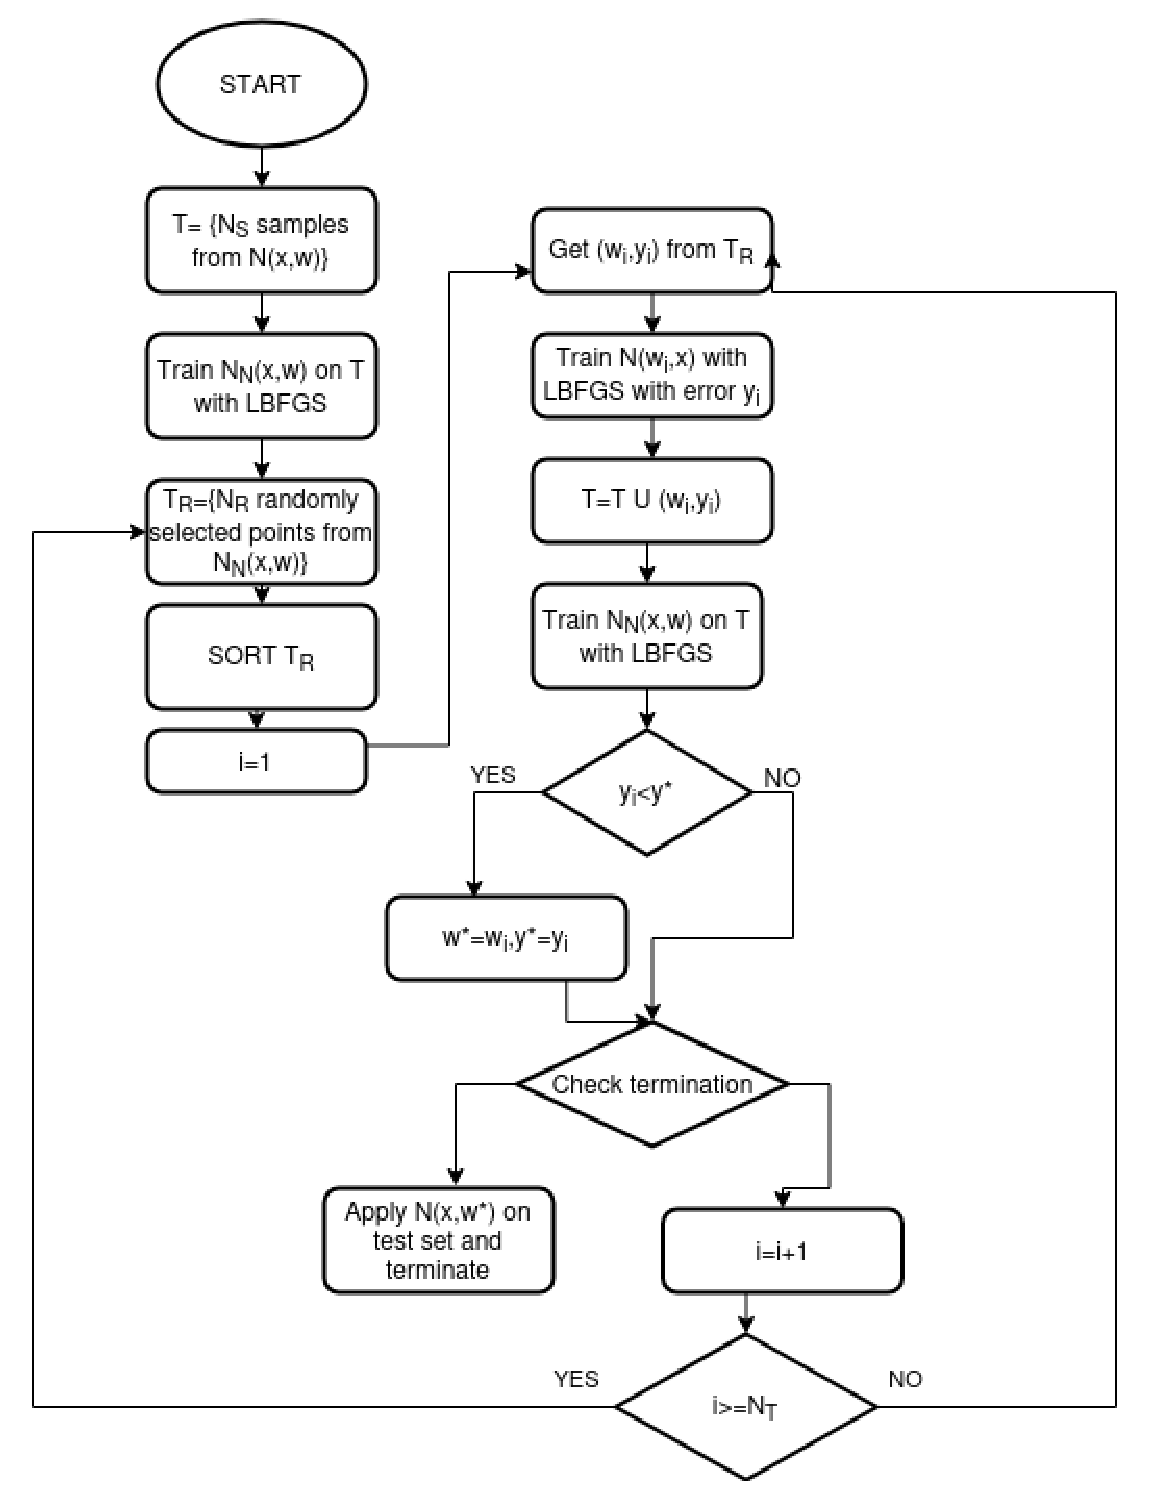
\includegraphics[scale=0.65]{diagram}
\par\end{centering}
\caption{The flowchart of the proposed method.\label{fig:flowchart}}

\end{figure}


\section{Experiments \label{sec:Experiments}}

The efficiency of the proposed artificial neural network training
technique was evaluated using a series of data sets from the relevant
literature. These datasets have been studied by various researchers
in the relevant literature and cover a wide range of research areas
from Physics to Economics. These datasets are are freely available
from the following websites:
\begin{enumerate}
\item The UCI repository, \url{https://archive.ics.uci.edu/}(accessed on
17 June 2023)\citep{uci}
\item The Keel repository, \url{https://sci2s.ugr.es/keel/datasets.php}(accessed
on 17 June 2023)\citep{Keel}.
\item The Statlib URL\textbf{ \url{ftp://lib.stat.cmu.edu/datasets/index.html }}(accessed
on 17 June 2023). This repository is used mainly for the regression
datasets.
\end{enumerate}

\subsection{Experimental datasets }

The following classification datasets from the relevant literature
were used in the experiments:
\begin{enumerate}
\item \textbf{Appendictis, }a dataset used for medical purposes and it was
found in \citep{appendicitis,appendicitis2}. 
\item \textbf{Australian} dataset \citep{australian}, an economic dataset,
related to bank transactions.
\item \textbf{Balance} dataset \citep{balance}, which is related to psychological
experiments.
\item \textbf{Cleveland} dataset, a medical dataset found in the following
research papers\citep{cleveland1,cleveland2}.
\item \textbf{Bands} dataset, related to printing problems \citep{bands}.
\item \textbf{Dermatology} dataset \citep{dermatology}, a dataset related
to dermatology problems.
\item \textbf{Hayes roth} dataset \citep{hayesroth}.
\item \textbf{Heart} dataset \citep{heart}, a medical dataset used to detect
heart diseases. 
\item \textbf{HouseVotes} dataset \citep{housevotes}, related to the Congressional
voting records of USA.
\item \textbf{Ionosphere} dataset, related to measurements from the ionosphere
an thoroughly studied in a series of research papers \citep{ion1,ion2}.
\item \textbf{Liverdisorder} dataset \citep{liver,liver1}, a medical dataset.
\item \textbf{Lymography} dataset \citep{lymography}.
\item \textbf{Mammographic} dataset \citep{mammographic}, a medical dataset
related to breast cancer diagnosis.
\item \textbf{Page Blocks }dataset \citep{pageblocks}.
\item \textbf{Parkinsons} dataset \citep{parkinsons1,parkinsons2}, a medical
dataset applied to the Parkinson's decease.
\item \textbf{Pima} dataset \citep{pima}, a medical dataset.
\item \textbf{Popfailures} dataset \citep{popfailures}, a dataset related
to meteorological data.
\item \textbf{Regions2} dataset, a medical dataset for liver biopsy images
\citep{regions}. 
\item \textbf{Saheart} dataset \citep{saheart}, a medical dataset related
to heart diseases. 
\item \textbf{Segment} dataset \citep{segment}, a dataset related to image
segmentation.
\item \textbf{Wdbc} dataset \citep{wdbc}, a dataset about breast tumors. 
\item \textbf{Wine} dataset, a dataset related to chemical analysis of wines
\citep{wine1,wine2}.
\item \textbf{Eeg} datasets \citep{eeg1,eeg2}, it is an EEG dataset and
the following cases were used in the experiments: 
\begin{enumerate}
\item Z\_F\_S, 
\item ZO\_NF\_S
\item ZONF\_S.
\end{enumerate}
\item \textbf{Zoo} dataset \citep{zoo}, suggested for to detect to proper
class of animals.
\end{enumerate}
A table showing the number of classes for every classification dataset
is shown in Table \ref{tab:classTable}.

\begin{table}[H]

\caption{Description for every classification dataset.\label{tab:classTable}}

\centering{}%
\begin{tabular}{|c|c|}
\hline 
DATASET & CLASSES\tabularnewline
\hline 
\hline 
Appendictis & 2\tabularnewline
\hline 
Australian & 2\tabularnewline
\hline 
Balance & 3\tabularnewline
\hline 
Cleveland & 5\tabularnewline
\hline 
Bands & 2\tabularnewline
\hline 
Dermatology & 6\tabularnewline
\hline 
Hayes Roth & 3\tabularnewline
\hline 
Heart & 2\tabularnewline
\hline 
Housevotes & 2\tabularnewline
\hline 
Ionosphere & 2\tabularnewline
\hline 
Liverdisorder & 2\tabularnewline
\hline 
Lymography & 4\tabularnewline
\hline 
Mammographic & 2\tabularnewline
\hline 
Page Blocks & 5\tabularnewline
\hline 
Parkinsons & 2\tabularnewline
\hline 
Pima & 2\tabularnewline
\hline 
Popfailures & 2\tabularnewline
\hline 
Regions2 & 5\tabularnewline
\hline 
Saheart & 2\tabularnewline
\hline 
Segment & 7\tabularnewline
\hline 
Wdbc & 2\tabularnewline
\hline 
Wine & 3\tabularnewline
\hline 
Z\_F\_S & 3\tabularnewline
\hline 
ZO\_NF\_S & 3\tabularnewline
\hline 
ZONF\_S & 2\tabularnewline
\hline 
Zoo & 7\tabularnewline
\hline 
\end{tabular}
\end{table}

The following regression datasets were used:
\begin{enumerate}
\item \textbf{Abalone} dataset \citep{abalone}, proposed to predict the
age of abalones.
\item \textbf{Airfoil }dataset, a dataset provided by NASA \citep{airfoil},
created from a series of aerodynamic and acoustic tests.
\item \textbf{Baseball} dataset, a dataset used to baseball games.
\item \textbf{BK} dataset \citep{Stat}, used to predict the points scored
in a basketball game. 
\item \textbf{BL} dataset, used in machine problems.
\item \textbf{Concrete} dataset \citep{concrete}, a dataset proposed to
calculate the concrete compressive strength
\item \textbf{Dee} dataset, used to detect the electricity energy prices.
\item \textbf{Diabetes} dataset, a medical dataset.
\item \textbf{Housing} dataset \citep{key23}.
\item \textbf{FA} dataset, used to fit body fat to other measurements. 
\item \textbf{MB} dataset \citep{key21}. 
\item \textbf{Mortgage} dataset. The goal is to predict the 30-Year Conventional
Mortgage Rate. 
\item \textbf{PY }dataset, (Pyrimidines problem)\citep{pydataset}.
\item \textbf{Quake} dataset, used to approximate the strength of a earthquake
given its the depth of its focal point, its latitude and its longitude. 
\item \textbf{Treasure} dataset, which contains Economic data information
of USA, where the goal is to predict 1-Month CD Rate. 
\item \textbf{Wankara} dataset, a weather dataset.
\end{enumerate}

\subsection{Experimental setup}

The proposed method was tested on the regression and classification
problems mentioned previously, and it was compared against the results
of several other well - known approaches of the relevant literature.
For greater reliability of the experimental results, the 10 - fold
validation technique was employed for every classification or regression
dataset. Every experiment was executed 30 times, with different initialization
for the random generator each time. Also, the srand48() random generator
of the C - programming language was utilized. The used code was implemented
in ANSI C++ using the freely available OPTIMUS optimization library
available from  \url{https://github.com/itsoulos/OPTIMUS/}. For the
case of classification datasets, the average classification error
is measured for every method and for regression datasets the average
mean squared error is measured in the test set. The number of hidden
nodes for the neural networks was set to $H=10$ for every method.
All the experiments were performed using an AMD Ryzen 5950X with 128GB
of RAM. The running operating system was Debian Linux. The methods
used in the experimental results are the following:
\begin{enumerate}
\item A genetic algorithm with 200 chromosomes used to train a neural network
with $H$ hidden nodes. This method was denoted as GENETIC in the
tables holding the experimental results. 
\item A Radial Basis Function (RBF) network \citep{rbf1} having $H$ hidden
nodes.
\item The Adam optimization method\citep{Adam}. Here the method is used
to minimize the train error of a neural network with $H$ hidden nodes.
\item The resilient back propagation (RPROP) optimization method\citep{rpropnn,rpropnn2,rpropnn3}
was employed also to train a neural network with $H$ hidden nodes.
\item The NEAT method (NeuroEvolution of Augmenting Topologies ) \citep{neat}.
\end{enumerate}
The values used for every parameter are listed in Table \ref{tab:Experimental-settings.}
and they are similar to the values used in the original publication
of the NeuralMinimizer method.

\begin{table}[H]
\caption{Experimental settings.\label{tab:Experimental-settings.}}

\centering{}%
\begin{tabular}{|c|c|c|}
\hline 
PARAMETER & MEANING & VALUE\tabularnewline
\hline 
\hline 
$H$ & Number of weights & 10\tabularnewline
\hline 
$N_{S}$ & Start samples & 50\tabularnewline
\hline 
$N_{T}$ & Starting points & 100\tabularnewline
\hline 
$N_{R}$ & Samples drawn from the first network & $10\times N_{T}$\tabularnewline
\hline 
$N_{G}$ & Maximum number of iterations & 200\tabularnewline
\hline 
\end{tabular}
\end{table}


\subsection{Experimental results}

The experimental results for the classification datasets are shown
in Table \ref{tab:tabClass} and for the regression datasets in Table
\ref{tab:exp2}. The column PROPOSED stands for the usage of the proposed
method to train a neural network with $H$ hidden nodes. In both tables,
the last row (denoted as AVERAGE) represents the mean error for each
method. Also, the figure \ref{fig:ScatterClass} shows a scatter plot
and the Wilcoxon signed-rank test for the classification datasets.
In the same direction, the figure \ref{fig:ScatterRegression} shows
the scatter plot for the regression datasets.

\begin{table}[H]
\caption{Experimental results for the classification datasets. The numbers
in cells denote average classification error of 30 independent runs.\label{tab:tabClass}}

\centering{}%
\begin{tabular}{|c|c|c|c|c|c|c|}
\hline 
DATASET & GENETIC & RBF & ADAM & RPROP & NEAT & PROPOSED\tabularnewline
\hline 
\hline 
Appendicitis & 18.10\% & 12.23\% & 16.50\% & 16.30\% & 17.20\% & 22.30\%\tabularnewline
\hline 
Australian & 32.21\% & 34.89\% & 35.65\% & 36.12\% & 31.98\% & 21.59\%\tabularnewline
\hline 
Balance & 8.97\% & 33.42\% & 7.87\% & 8.81\% & 23.14\% & 5.46\%\tabularnewline
\hline 
Bands & 35.75\% & 37.22\% & 36.25\% & 36.32\% & 34.30\% & 33.06\%\tabularnewline
\hline 
Cleveland & 51.60\% & 67.10\% & 67.55\% & 61.41\% & 53.44\% & 45.41\%\tabularnewline
\hline 
Dermatology & 30.58\% & 62.34\% & 26.14\% & 15.12\% & 32.43\% & 4.14\%\tabularnewline
\hline 
Hayes Roth & 56.18\% & 64.36\% & 59.70\% & 37.46\% & 50.15\% & 35.28\%\tabularnewline
\hline 
Heart & 28.34\% & 31.20\% & 38.53\% & 30.51\% & 39.27\% & 17.93\%\tabularnewline
\hline 
HouseVotes & 6.62\% & 6.13\% & 7.48\% & 6.04\% & 10.89\% & 5.78\%\tabularnewline
\hline 
Ionosphere & 15.14\% & 16.22\% & 16.64\% & 13.65\% & 19.67\% & 16.31\%\tabularnewline
\hline 
Liverdisorder & 31.11\% & 30.84\% & 41.53\% & 40.26\% & 30.67\% & 33.02\%\tabularnewline
\hline 
Lymography & 23.26\% & 25.31\% & 29.26\% & 24.67\% & 33.70\% & 25.64\%\tabularnewline
\hline 
Mammographic & 19.88\% & 21.38\% & 46.25\% & 18.46\% & 22.85\% & 16.37\%\tabularnewline
\hline 
PageBlocks & 8.06\% & 10.09\% & 7.93\% & 7.82\% & 10.22\% & 5.44\%\tabularnewline
\hline 
Parkinsons & 18.05\% & 17.42\% & 24.06\% & 22.28\% & 18.56\% & 14.47\%\tabularnewline
\hline 
Pima & 32.19\% & 25.78\% & 34.85\% & 34.27\% & 34.51\% & 25.61\%\tabularnewline
\hline 
Popfailures & 5.94\% & 7.04\% & 5.18\% & 4.81\% & 7.05\% & 5.57\%\tabularnewline
\hline 
Regions2 & 29.39\% & 38.29\% & 29.85\% & 27.53\% & 33.23\% & 22.73\%\tabularnewline
\hline 
Saheart & 34.86\% & 32.19\% & 34.04\% & 34.90\% & 34.51\% & 34.03\%\tabularnewline
\hline 
Segment & 57.72\% & 59.68\% & 49.75\% & 52.14\% & 66.72\% & 37.28\%\tabularnewline
\hline 
Wdbc & 8.56\% & 7.27\% & 35.35\% & 21.57\% & 12.88\% & 5.01\%\tabularnewline
\hline 
Wine & 19.20\% & 31.41\% & 29.40\% & 30.73\% & 25.43\% & 7.14\%\tabularnewline
\hline 
Z\_F\_S & 10.73\% & 13.16\% & 47.81\% & 29.28\% & 38.41\% & 7.09\%\tabularnewline
\hline 
ZO\_NF\_S & 8.41\% & 9.02\% & 47.43\% & 6.43\% & 43.75\% & 5.15\%\tabularnewline
\hline 
ZONF\_S & 2.60\% & 4.03\% & 11.99\% & 27.27\% & 5.44\% & 2.35\%\tabularnewline
\hline 
ZOO & 16.67\% & 21.93\% & 14.13\% & 15.47\% & 20.27\% & 4.20\%\tabularnewline
\hline 
\textbf{AVERAGE} & \textbf{23.47\%} & \textbf{27.69\%} & \textbf{30.81\%} & \textbf{25.37\%} & \textbf{28.87\%} & \textbf{17.63\%}\tabularnewline
\hline 
\end{tabular}
\end{table}
\begin{table}[H]
\caption{Average regression error for the regression datasets. \label{tab:exp2}}

\centering{}%
\begin{tabular}{|c|c|c|c|c|c|c|}
\hline 
DATASET & GENETIC & RBF & ADAM & RPROP & NEAT & PROPOSED\tabularnewline
\hline 
\hline 
ABALONE & 7.17 & 7.37 & 4.30 & 4.55 & 9.88 & 4.50\tabularnewline
\hline 
AIRFOIL & 0.003 & 0.27 & 0.005 & 0.002 & 0.067 & 0.003\tabularnewline
\hline 
BASEBALL & 103.60 & 93.02 & 77.90 & 92.05 & 100.39 & 56.16\tabularnewline
\hline 
BK & 0.027 & 0.02 & 0.03 & 1.599 & 0.15 & 0.02\tabularnewline
\hline 
BL & 5.74 & 0.01 & 0.28 & 4.38 & 0.05 & 0.0004\tabularnewline
\hline 
CONCRETE & 0.0099 & 0.011 & 0.078 & 0.0086 & 0.081 & 0.003\tabularnewline
\hline 
DEE & 1.013 & 0.17 & 0.63 & 0.608 & 1.512 & 0.30\tabularnewline
\hline 
DIABETES & 19.86 & 0.49 & 3.03 & 1.11 & 4.25 & 1.24\tabularnewline
\hline 
HOUSING & 43.26 & 57.68 & 80.20 & 74.38 & 56.49 & 18.30\tabularnewline
\hline 
FA & 1.95 & 0.02 & 0.11 & 0.14 & 0.19 & 0.01\tabularnewline
\hline 
MB & 3.39 & 2.16 & 0.06 & 0.055 & 0.061 & 0.05\tabularnewline
\hline 
MORTGAGE & 2.41 & 1.45 & 9.24 & 9.19 & 14.11 & 3.50\tabularnewline
\hline 
PY & 105.41 & 0.02 & 0.09 & 0.039 & 0.075 & 0.03\tabularnewline
\hline 
QUAKE & 0.04 & 0.071 & 0.06 & 0.041 & 0.298 & 0.039\tabularnewline
\hline 
TREASURY & 2.929 & 2.02 & 11.16 & 10.88 & 15.52 & 3.72\tabularnewline
\hline 
WANKARA & 0.012 & 0.001 & 0.02 & 0.0003 & 0.005 & 0.002\tabularnewline
\hline 
\textbf{AVERAGE} & \textbf{18.55} & \textbf{10.30} & \textbf{11.70} & \textbf{12.44} & \textbf{12.70} & \textbf{5.49}\tabularnewline
\hline 
\end{tabular}
\end{table}
\begin{figure}[H]
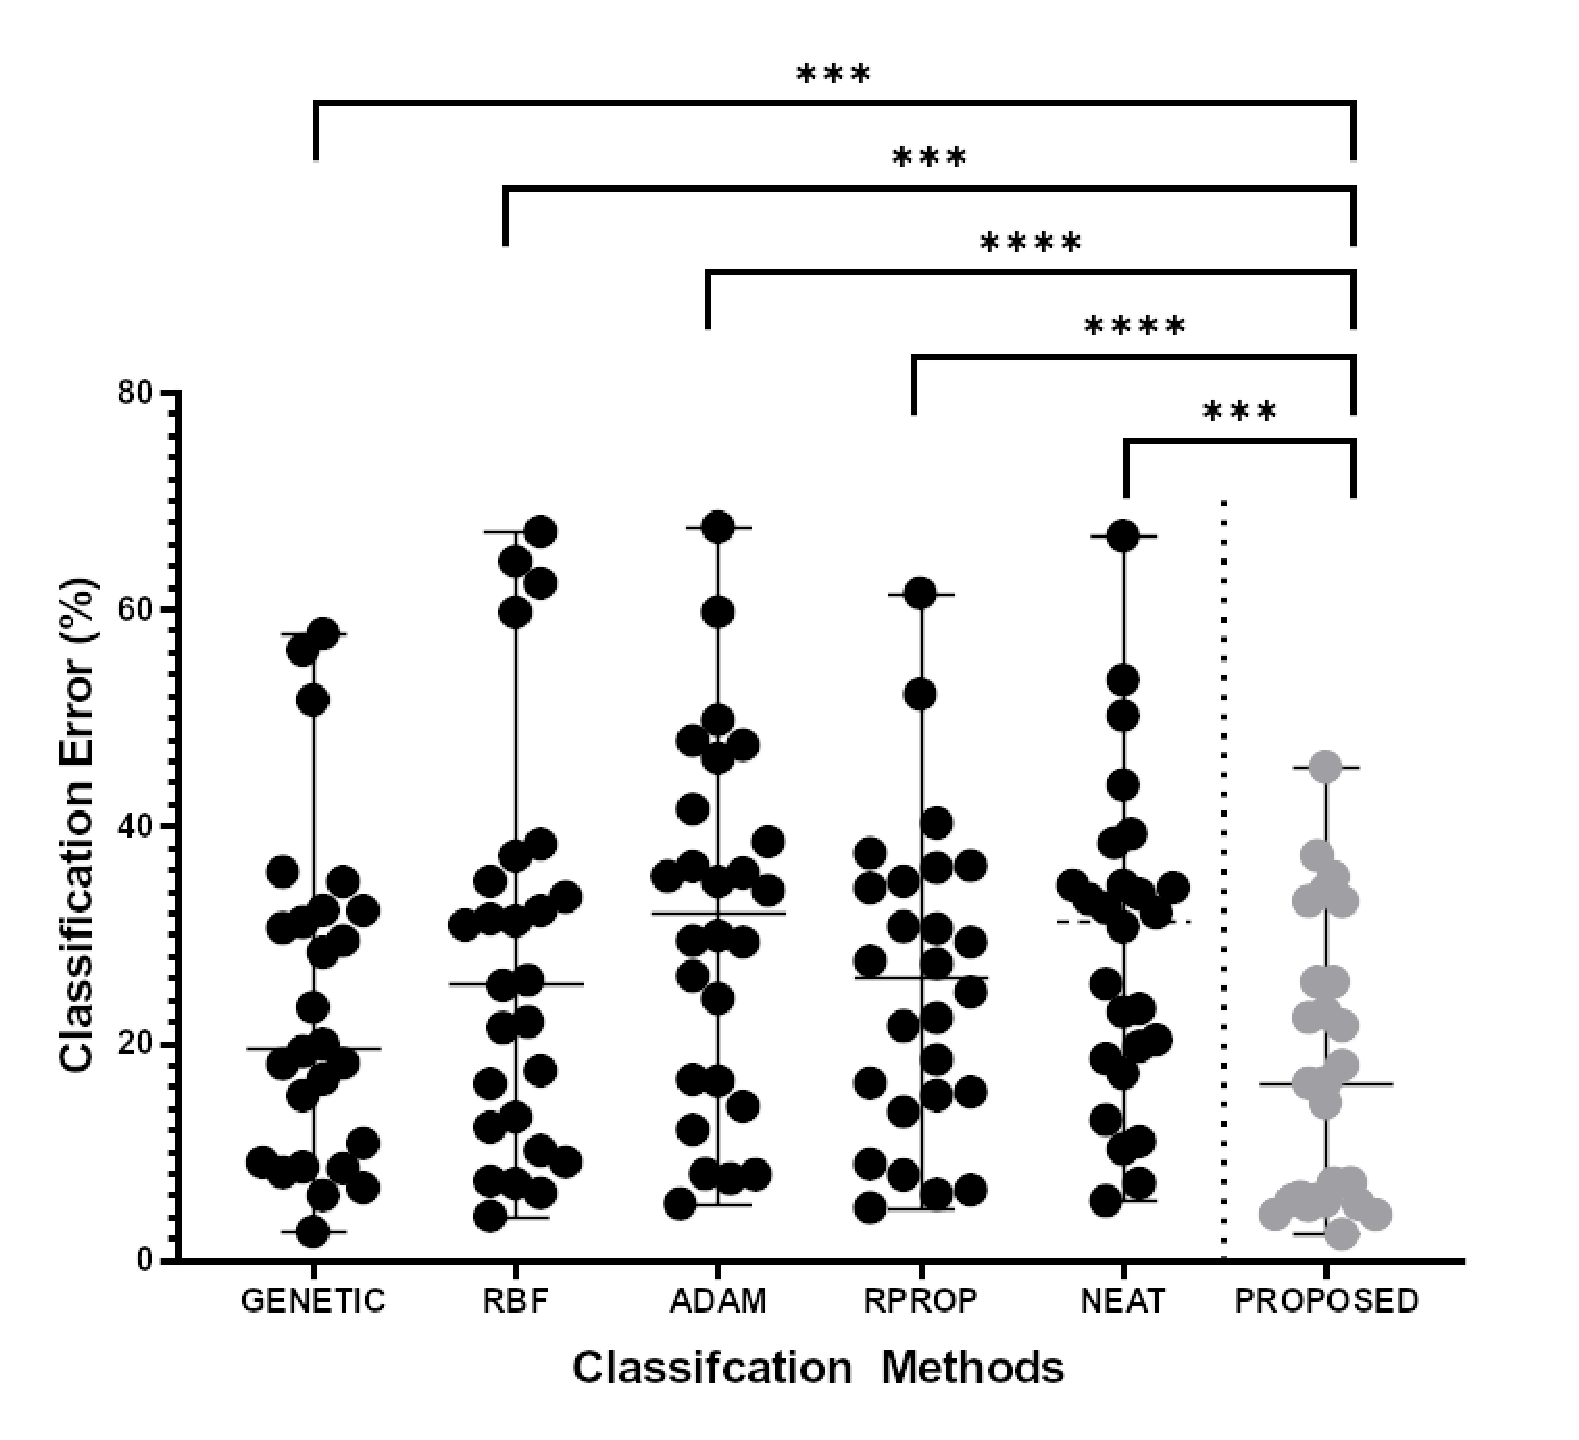
\includegraphics[scale=0.45]{nmin_class}

\caption{Scatter plot representation and the Wilcoxon signed-rank test results
of the comparison for each of the five (5) classification methods
(GENETIC, RBF, ADAM, RPROP, NEAT) with the PROPOSED method regarding
the classification error in twenty-six (26) different public available
classification datasets. Star links join significantly different values;
three stars ({*}{*}{*}) stand for p\textless 0.001. \label{fig:ScatterClass}}

\end{figure}
\begin{figure}[H]
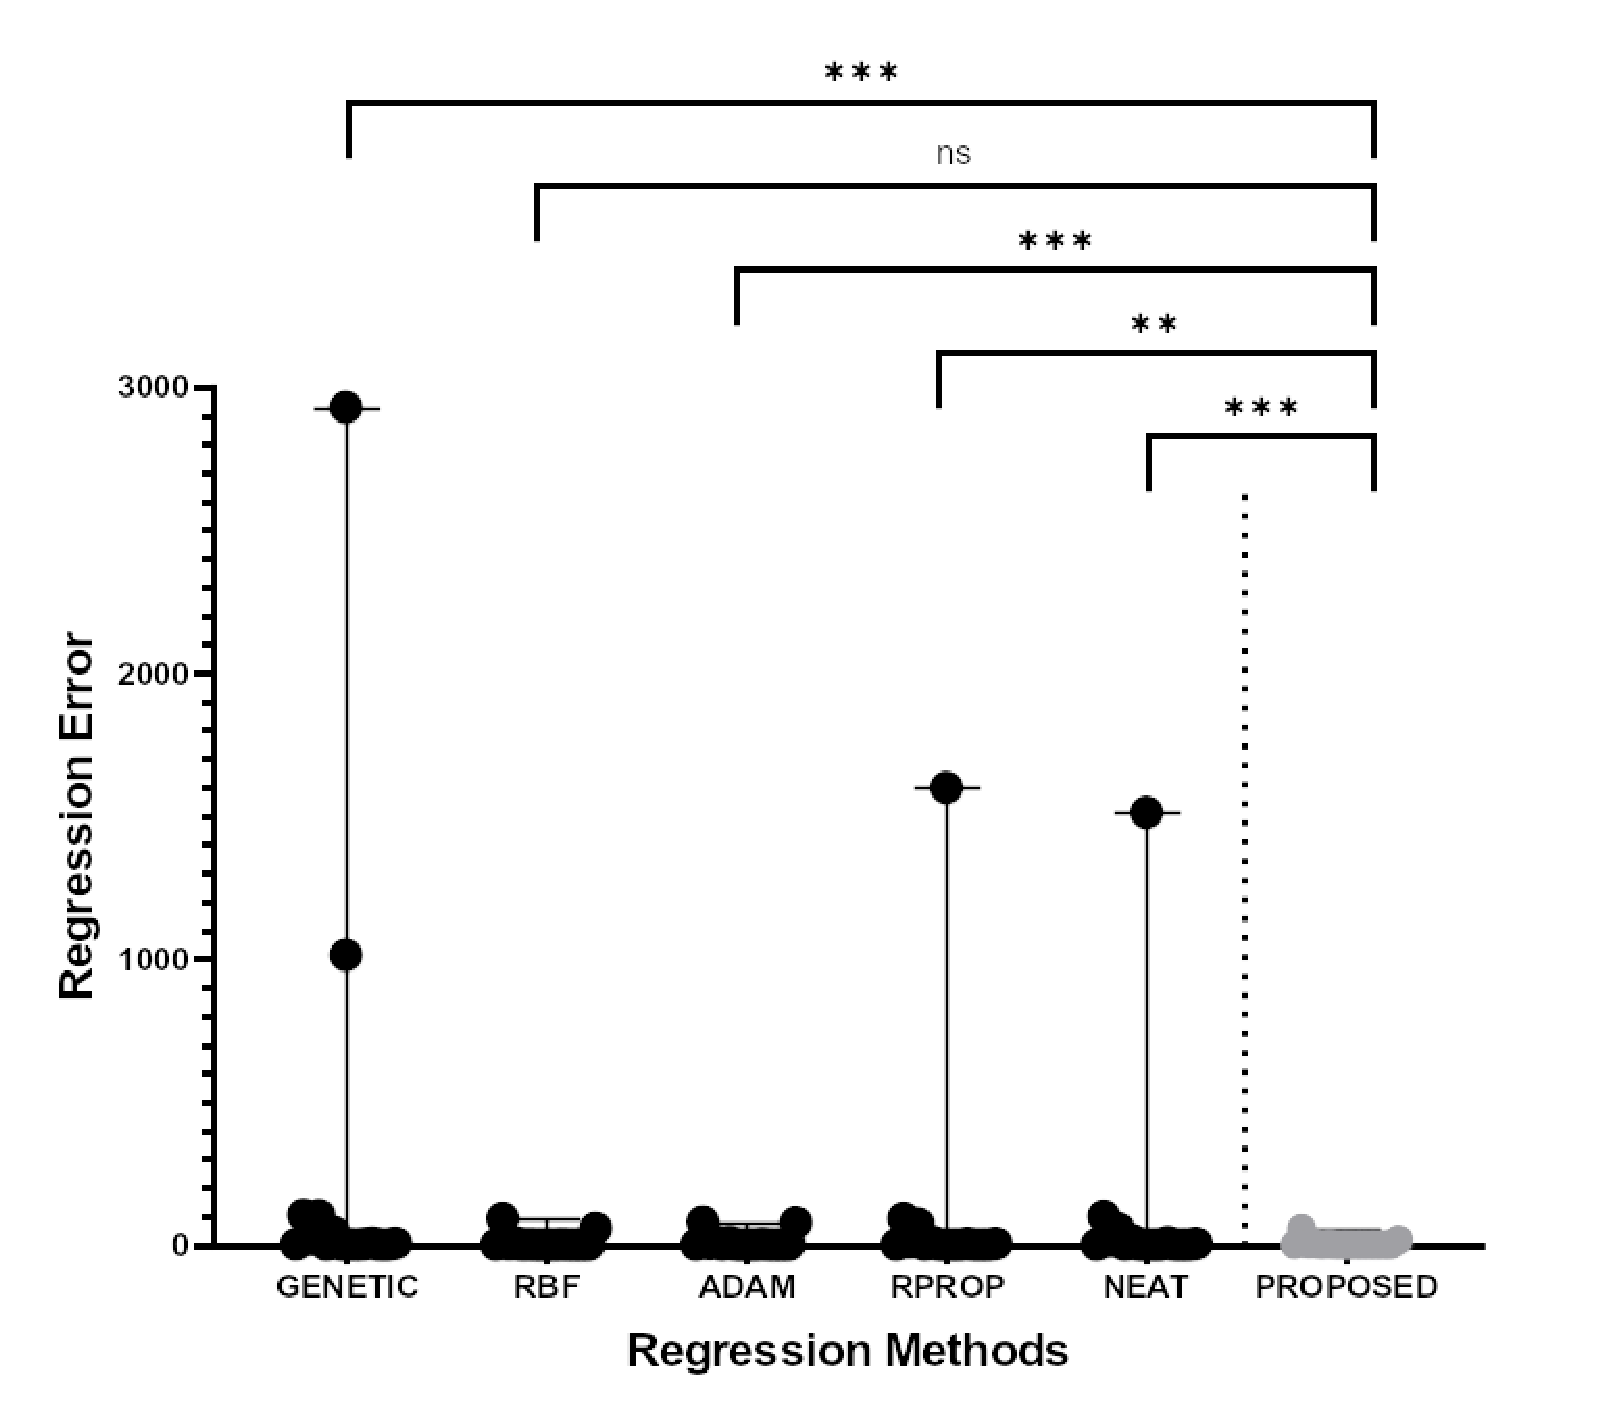
\includegraphics[scale=0.45]{nmin_regression}

\caption{Scatter plot representation and the Wilcoxon signed-rank test results
of the comparison for each of the five (5) regression methods (GENETIC,
RBF, ADAM, RPROP, NEAT) with the PROPOSED method regarding the regression
error in sixteen (16) different publicly available classification
datasets. Star links join significantly different values; three stars
({*}{*}{*}) stand for p\textless 0.001. The notation \textquotedbl ns\textquotedbl{}
denotes \textquotedbl not significant\textquotedbl .\label{fig:ScatterRegression}}

\end{figure}
The experimental results and their graphical representation demonstrate
the superiority of the proposed technique over the others in terms
of the average error, as measured in the test set. For example, in
the case of datasets used for classification, the proposed method
outperforms the remaining techniques in 19 out of 26 datasets (73\%
percent). Also, in several cases, the percentage reduction in error
exceeds 50\%. For the classification problems, the immediate most
effective training method after the proposed one is the genetic algorithm
and, on average, the proposed technique achieves lower classification
error than the genetic algorithm error by 24\%. Moreover, in regression
problems, the next most effective method after the proposed one is
the RBF neural network with small differences from the ADAM optimizer.
However, in the case of regression problems, the improvement in average
error by using the proposed technique exceeds 49\%. Of course, the
proposed technique is quite time-consuming since it requires continuous
training of an artificial neural network. 

\section{Conclusions\label{sec:Conclusions}}

In this work, the application of a recent global minimization method
for the training of artificial neural networks was proposed. The application
of this method was used in artificial neural networks both for classification
problems and for regression problems. This new global minimization
method constructs an approximation of the objective function using
neural networks. This construction is done with a limited number of
samples from the objective function. However, each time a local minimization
takes place, this approximation is readjusted. Subsequently, the sampling
for the minimization is done from the approximate function and not
from the objective one, even taking samples from the approximation
with the smallest function value, in order to speed up the finding
of the global minimum. In this particular case, the artificial neural
network of the global minimization method is used to train the artificial
neural network. However, due to the large time and storage requirements
of artificial neural networks, the RBF network of the original NeuralMinimizer
method was replaced with an artificial neural network that was trained
using the local minimization method L-BFGS. The new artificial neural
network training technique is tested on a wide collection of classification
and regression problems from the relevant literature and is shown
to significantly improve the learning error over other established
artificial neural network training techniques. This improvement is
25\% on average for the case of classification problems and rises
significantly to 50\% for regression problems.

Nevertheless, the proposed procedure can be extremely slow, especially
as the size of the artificial neural network increases. The size of
the artificial neural network directly depends on the dimension of
the input dataset. Future improvements to the methodology may include
the use of parallel programming techniques, such as parallel implementations
of the L-BFGS optimization method, in order to accelerate the training
of artificial neural networks by taking advantage of modern computing
structures. Also, in the present phase, as a minimization method in
step \ref{enu:Optimization-Step.} of the proposed training method,
a local minimization method is used. Future extensions could explore
the possibility of also using global minimization techniques in this
step, although care should be taken to make use of parallel computing
techniques to avoid long execution times.

\vspace{6pt}


\authorcontributions{I.G.T. and A.T. conceived of the idea and the methodology and I.G.T
has implemented the corresponding software. I.G.T. conducted the experiments,
employing objective functions as test cases, and provided the comparative
experiments. A.T. has performed the necessary statistical tests. All
authors have read and agreed to the published version of the manuscript.}

\funding{This research received no external funding.}

\institutionalreview{Not applicable.}

\informedconsent{Not applicable. }

\institutionalreview{Not applicable.}

\acknowledgments{This research has been co-financed by the European Regional Development
Fund of the European Union and Greek national funds through the Operational
Program Competitiveness, Entrepreneurship and Innovation, under the
call Research -Create-Innovate, project name “Create a system of recommendations
and augmented reality applications in a hotel\textquotedbl{} (project
code:T1EDK-03745). }

\sampleavailability{Not applicable.}

\appendixtitles{no}

\appendixstart{}

\appendix

\begin{adjustwidth}{-\extralength}{0cm}{}

\reftitle{References}
\begin{thebibliography}{99}
\bibitem{nn1}C. Bishop, Neural Networks for Pattern Recognition,
Oxford University Press, 1995.

\bibitem{nn2}G. Cybenko, Approximation by superpositions of a sigmoidal
function, Mathematics of Control Signals and Systems \textbf{2}, pp.
303-314, 1989.

\bibitem{nnreview}O.I. Abiodun, A. Jantan, A. E. Omolara, K.V. Dada,
N. A. Mohamed, H. Arshad, State-of-the-art in artificial neural network
applications: A survey, Heliyon \textbf{4}, e00938, 2018.

\bibitem{nnphysics1}P. Baldi, K. Cranmer, T. Faucett et al, Parameterized
neural networks for high-energy physics, Eur. Phys. J. C \textbf{76},
2016.

\bibitem{nnphysics2}J. J. Valdas and G. Bonham-Carter, Time dependent
neural network models for detecting changes of state in complex processes:
Applications in earth sciences and astronomy, Neural Networks \textbf{19},
pp. 196-207, 2006

\bibitem{nnphysics3}G. Carleo,M. Troyer, Solving the quantum many-body
problem with artificial neural networks, Science \textbf{355}, pp.
602-606, 2017.

\bibitem{nnchem1}Lin Shen, Jingheng Wu, and Weitao Yang, Multiscale
Quantum Mechanics/Molecular Mechanics Simulations with Neural Networks,
Journal of Chemical Theory and Computation \textbf{12}, pp. 4934-4946,
2016.

\bibitem{nnchem2}Sergei Manzhos, Richard Dawes, Tucker Carrington,
Neural network‐based approaches for building high dimensional and
quantum dynamics‐friendly potential energy surfaces, Int. J. Quantum
Chem. \textbf{115}, pp. 1012-1020, 2015.

\bibitem{nnchem3}Jennifer N. Wei, David Duvenaud, and Alán Aspuru-Guzik,
Neural Networks for the Prediction of Organic Chemistry Reactions,
ACS Central Science \textbf{2}, pp. 725-732, 2016.

\bibitem{nnecon1}Lukas Falat and Lucia Pancikova, Quantitative Modelling
in Economics with Advanced Artificial Neural Networks, Procedia Economics
and Finance \textbf{34}, pp. 194-201, 2015.

\bibitem{nnecon2}Mohammad Namazi, Ahmad Shokrolahi, Mohammad Sadeghzadeh
Maharluie, Detecting and ranking cash flow risk factors via artificial
neural networks technique, Journal of Business Research \textbf{69},
pp. 1801-1806, 2016.

\bibitem{nncecon3}G. Tkacz, Neural network forecasting of Canadian
GDP growth, International Journal of Forecasting \textbf{17}, pp.
57-69, 2001.

\bibitem{nnmed1}Igor I. Baskin, David Winkler and Igor V. Tetko,
A renaissance of neural networks in drug discovery, Expert Opinion
on Drug Discovery \textbf{11}, pp. 785-795, 2016.

\bibitem{nnmed2}Ronadl Bartzatt, Prediction of Novel Anti-Ebola Virus
Compounds Utilizing Artificial Neural Network (ANN), Chemistry Faculty
Publications \textbf{49}, pp. 16-34, 2018.

\bibitem{nnde1}I. E. Lagaris, A. Likas, D. I. Fotiadis, Artificial
neural networks for solving ordinary and partial differential equations,
IEEE Transactions on Neural Networks \textbf{9}, pp. 987-1000, 1998.

\bibitem{nnde2}S. Effati, M. Pakdaman, Artificial neural network
approach for solving fuzzy differential equations, Information Sciences
\textbf{180}, pp. 1434-1457, 2010.

\bibitem{nnde3}F. Rostami, A. Jafarian, A new artificial neural network
structure for solving high-order linear fractional differential equations,
International Journal of Computer Mathematics \textbf{95}, pp. 528-539,
2018.

\bibitem{nnsolar1}A.K. Yadav, S.S. Chandel, Solar radiation prediction
using Artificial Neural Network techniques: A review, Renewable and
Sustainable Energy Reviews \textbf{33}, pp 772-781, 2014.

\bibitem{nnsolar2}A. Qazi, H. Fayaz, A. Wadi, R.G. Raj, N.A. Rahim,
W.A. Khan, The artificial neural network for solar radiation prediction
and designing solar systems: a systematic literature review, Journal
of Cleaner Production \textbf{104}, pp 1-12, 2015.

\bibitem{nnspam1}C.H. Wu, Behavior-based spam detection using a hybrid
method of rule-based techniques and neural networks, Expert Systems
with Applications \textbf{36}, pp. 4321-4330, 2009.

\bibitem{nnspam2}Y. Ren, D. Ji, Neural networks for deceptive opinion
spam detection: An empirical study, Information Sciences \textbf{385--386},
pp. 213-224, 2017.

\bibitem{nnspam3}S. Madisetty, M.S. Desarkar, A Neural Network-Based
Ensemble Approach for Spam Detection in Twitter, IEEE Transactions
on Computational Social Systems \textbf{ 5}, pp. 973-984, 2018.

\bibitem{nnagr1}A. Topuz, Predicting moisture content of agricultural
products using artificial neural networks, Advances in Engineering
Software \textbf{41}, pp. 464-470, 2010.

\bibitem{nnagr2}A. Escamilla-García, G.M. Soto-Zarazúa, M. Toledano-Ayala,
E. Rivas-Araiza, A. Gastélum-Barrios, Abraham,Applications of Artificial
Neural Networks in Greenhouse Technology and Overview for Smart Agriculture
Development, Applied Sciences \textbf{10}, Article number 3835, 2020.

\bibitem{nnfacial}H. Boughrara, M. Chtourou, C. Ben Amar et al, Facial
expression recognition based on a mlp neural network using constructive
training algorithm. Multimed Tools Appl \textbf{75}, pp. 709--731,
2016.

\bibitem{nnwind}H. Liu, H.Q Tian, Y.F. Li, L. Zhang, Comparison of
four Adaboost algorithm based artificial neural networks in wind speed
predictions, Energy Conversion and Management \textbf{92}, pp. 67-81,
2015.

\bibitem{nngas}J. Szoplik, Forecasting of natural gas consumption
with artificial neural networks, Energy \textbf{85}, pp. 208-220,
2015.

\bibitem{nnintrusion}H. Bahram, N.J. Navimipour, Intrusion detection
for cloud computing using neural networks and artificial bee colony
optimization algorithm, ICT Express 5, pp. 56-59, 2019.

\bibitem{nnhydro1}Y.S. Chen, F.J. Chang, Evolutionary artificial
neural networks for hydrological systems forecasting, Journal of Hydrology
\textbf{367}, pp. 125-137, 2009.

\bibitem{nninvest}G.S. Swales, Y.Yoon, Applying Artificial Neural
Networks to Investment Analysis, Financial Analysts Journal \textbf{48},
pp. 78-80, 1992.

\bibitem{bpnn}D.E. Rumelhart, G.E. Hinton and R.J. Williams, Learning
representations by back-propagating errors, Nature \textbf{323}, pp.
533 - 536 , 1986.

\bibitem{bpnn2}T. Chen and S. Zhong, Privacy-Preserving Backpropagation
Neural Network Learning, IEEE Transactions on Neural Networks \textbf{20},
, pp. 1554-1564, 2009.

\bibitem{nnhill}S. Chalup, F. Maire, A study on hill climbing algorithms
for neural network training, In: Proceedings of the 1999 Congress
on Evolutionary Computation-CEC99 (Cat. No. 99TH8406), Washington,
DC, USA, 1999, pp. 2014-2021 Vol. 3.

\bibitem{rpropnn}M. Riedmiller and H. Braun, A Direct Adaptive Method
for Faster Backpropagation Learning: The RPROP algorithm, Proc. of
the IEEE Intl. Conf. on Neural Networks, San Francisco, CA, pp. 586--591,
1993.

\bibitem{rpropnn3}T. Pajchrowski, K. Zawirski and K. Nowopolski,
Neural Speed Controller Trained Online by Means of Modified RPROP
Algorithm, IEEE Transactions on Industrial Informatics \textbf{11},
pp. 560-568, 2015.

\bibitem{rpropnn2}Rinda Parama Satya Hermanto, Suharjito, Diana,
Ariadi Nugroho, Waiting-Time Estimation in Bank Customer Queues using
RPROP Neural Networks, Procedia Computer Science \textbf{ 135}, pp.
35-42, 2018.

\bibitem{key-23}Neural Networks, Procedia Computer Science \textbf{ 135},
pp. 35-42, 2018.

\bibitem{quasinn}B. Robitaille and B. Marcos and M. Veillette and
G. Payre, Modified quasi-Newton methods for training neural networks,
Computers \& Chemical Engineering \textbf{20}, pp. 1133-1140, 1996.

\bibitem{quasinn2}Q. Liu, J. Liu, R. Sang, J. Li, T. Zhang and Q.
Zhang, Fast Neural Network Training on FPGA Using Quasi-Newton Optimization
Method,IEEE Transactions on Very Large Scale Integration (VLSI) Systems
\textbf{26}, pp. 1575-1579, 2018.

\bibitem{nn_ann1}A. Yamazaki, M. C. P. de Souto,T. B. Ludermir, Optimization
of neural network weights and architectures for odor recognition using
simulated annealing, In: Proceedings of the 2002 International Joint
Conference on Neural Networks. IJCNN'02 \textbf{1}, pp. 547-552 ,
2002.

\bibitem{nn_ann2}Y. Da, G. Xiurun, An improved PSO-based ANN with
simulated annealing technique, Neurocomputing \textbf{63}, pp. 527-533,
2005.

\bibitem{geneticnn}F. H. F. Leung, H. K. Lam, S. H. Ling and P. K.
S. Tam, Tuning of the structure and parameters of a neural network
using an improved genetic algorithm, IEEE Transactions on Neural Networks
\textbf{14}, pp. 79-88, 2003

\bibitem{geneticnn2}X. Yao, Evolving artificial neural networks,
Proceedings of the IEEE, 87(9), pp. 1423-1447, 1999.

\bibitem{psonn}C. Zhang, H. Shao and Y. Li, Particle swarm optimisation
for evolving artificial neural network, IEEE International Conference
on Systems, Man, and Cybernetics, , pp. 2487-2490, 2000.

\bibitem{psonn2}Jianbo Yu, Shijin Wang, Lifeng Xi, Evolving artificial
neural networks using an improved PSO and DPSO \textbf{71}, pp. 1054-1060,
2008.

\bibitem{nndem}J. Ilonen, J.K. Kamarainen, J. Lampinen, Differential
Evolution Training Algorithm for Feed-Forward Neural Networks, Neural
Processing Letters \textbf{17}, pp. 93--105, 2003.

\bibitem{nndem2}A. Slowik, M. Bialko, Training of artificial neural
networks using differential evolution algorithm, In: 2008 Conference
on Human System Interactions, Krakow, Poland, pp. 60-65, 2008.

\bibitem{nnevo}M. Rocha, P. Cortez, J. Neves, Evolution of neural
networks for classification and regression, Neurocomputing \textbf{70},
pp. 2809-2816, 2007.

\bibitem{nnwhale}I. Aljarah, H. Faris, S. Mirjalili, Optimizing connection
weights in neural networks using the whale optimization algorithm,
Soft Comput \textbf{22}, pp. 1--15, 2018.

\bibitem{nnplant}Z. Cui , C. Yang, S. Sanyal, Training artificial
neural networks using APPM, International Journal of Wireless and
Mobile Computing \textbf{ 5}, pp. 168-174, 2012.

\bibitem{nnbird}A. Askarzadeh, A. Rezazadeh, Artificial neural network
training using a new efficient optimization algorithm, Applied Soft
Computing \textbf{13}, pp 1206-1213, 2013.

\bibitem{nnhybrid2}J.F. Chen, Q.H. Do,H.N. Hsieh, Training Artificial
Neural Networks by a Hybrid PSO-CS Algorithm, Algorithms \textbf{8},
pp. 292-308, 2015.

\bibitem{nnhybrid1}M. Yaghini, M.M. Khoshraftar, M. Fallahi, A hybrid
algorithm for artificial neural network training, Engineering Applications
of Artificial Intelligence \textbf{26}, pp 293-301, 2013.

\bibitem{csmethod}X.S. Yang, S. Deb, Engineering Optimisation by
Cuckoo Search, Int. J. Math. Model. Numer. Optim. \textbf{1}, 330--343,
2010.

\bibitem{nninit1}I. Ivanova, M. Kubat, Initialization of neural networks
by means of decision trees, Knowledge-Based Systems \textbf{8}, pp.
333-344, 1995.

\bibitem{weight_init2}J.Y.F. Yam, T.W.S. Chow, A weight initialization
method for improving training speed in feedforward neural network,
Neurocomputing \textbf{30}, pp. 219-232, 2000.

\bibitem{weight_init3}K. Chumachenko, A. Iosifidis, M. Gabbouj, Feedforward
neural networks initialization based on discriminant learning, Neural
Networks \textbf{146}, pp. 220-229, 2022.

\bibitem{nninit2}F. Itano, M. A. de Abreu de Sousa, E. Del-Moral-Hernandez,
Extending MLP ANN hyper-parameters Optimization by using Genetic Algorithm,
In: 2018 International Joint Conference on Neural Networks (IJCNN),
Rio de Janeiro, Brazil, 2018, pp. 1-8, 2018.

\bibitem{nninit3}F. Itano, M. A. de Abreu de Sousa, E. Del-Moral-Hernandez,
Extending MLP ANN hyper-parameters Optimization by using Genetic Algorithm,\textquotedbl{}
2018 International Joint Conference on Neural Networks (IJCNN), Rio
de Janeiro, Brazil, pp. 1-8, 2018.

\bibitem{nninitreview}M.V. Narkhede, P.P. Bartakke, M.S. Sutaone,
A review on weight initialization strategies for neural networks,
Artif Intell Rev \textbf{55}, pp. 291--322, 2022.

\bibitem{nngencon}F. H. F. Leung, H. K. Lam, S. H. Ling, P. K. S.
Tam, Tuning of the structure and parameters of a neural network using
an improved genetic algorithm, IEEE Transactions on Neural Networks
\textbf{14}, pp. 79-88, 2003.

\bibitem{mainGe}M. O’Neill, C. Ryan, Grammatical evolution, IEEE
Trans. Evol. Comput. \textbf{5}, pp. 349--358, 2001.

\bibitem{nnc}I.G. Tsoulos, D. Gavrilis, E. Glavas, Neural network
construction and training using grammatical evolution, Neurocomputing
72, pp. 269-277, 2008.

\bibitem{nnprunncon}H.G. Han, J.F. Qiao, A structure optimisation
algorithm for feedforward neural network construction, Neurocomputing
\textbf{99}, pp 347-357, 2013.

\bibitem{nncell}K.J. Kim, S.B. Cho, Evolved neural networks based
on cellular automata for sensory-motor controller, Neurocomputing
\textbf{69}, pp. 2193-2207, 2006.

\bibitem{weight_gpu1}M. Martínez-Zarzuela, F.J. Díaz Pernas, J.F.
Díez Higuera, M.A. Rodríguez, Fuzzy ART Neural Network Parallel Computing
on the GPU. In: Sandoval, F., Prieto, A., Cabestany, J., Graña, M.
(eds) Computational and Ambient Intelligence. IWANN 2007. Lecture
Notes in Computer Science, vol 4507. Springer, Berlin, Heidelberg,
2007.

\bibitem{weight_gpu2}X. Sierra-Canto, F. Madera-Ramirez, V. Uc-Cetina,
Parallel Training of a Back-Propagation Neural Network Using CUDA,
In: 2010 Ninth International Conference on Machine Learning and Applications,
Washington, DC, USA, pp. 307-312, 2010.

\bibitem{weight_gpu3}A.A. Huqqani, E. Schikuta, S. Ye Peng Chen,
Multicore and GPU Parallelization of Neural Networks for Face Recognition,
Procedia Computer Science \textbf{18}, pp. 349-358, 2013.

\bibitem{nnsharing1}S.J. Nowlan and G.E. Hinton, Simplifying neural
networks by soft weight sharing, Neural Computation 4, pp. 473-493,
1992.

\bibitem{nnsharing2}J.K. Kim, M.Y. Lee, J.Y. Kim, B. J. Kim, J. H.
Lee, An efficient pruning and weight sharing method for neural network,
In: 2016 IEEE International Conference on Consumer Electronics-Asia
(ICCE-Asia), Seoul, Korea (South), pp. 1-2, 2016.

\bibitem{nnprunning1}S.J. Hanson and L.Y. Pratt, Comparing biases
for minimal network construction with back propagation, In D.S. Touretzky
(Ed.), Advances in Neural Information Processing Systems, Volume 1,
pp. 177-185, San Mateo, CA: Morgan Kaufmann, 1989.

\bibitem{nnprunning2}M.C. Mozer and P. Smolensky, Skeletonization:
a technique for trimming the fat from a network via relevance assesment.
In D.S. Touretzky (Ed.), Advances in Neural Processing Systems, Volume
1, pp. 107-115, San Mateo CA: Morgan Kaufmann, 1989.

\bibitem{nnprunning3}M. Augasta and T. Kathirvalavakumar, Pruning
algorithms of neural networks --- a comparative study, Central European
Journal of Computer Science, 2003.

\bibitem{nndrop1}Nitish Srivastava, G E Hinton, Alex Krizhevsky,
Ilya Sutskever, Ruslan R Salakhutdinov, Dropout: a simple way to prevent
neural networks from overfitting, Journal of Machine Learning Research
\textbf{15}, pp. 1929-1958, 2014.

\bibitem{nndrop2}A. Iosifidis, A. Tefas, I. Pitas, DropELM: Fast
neural network regularization with Dropout and DropConnect, Neurocomputing
\textbf{162}, pp. 57-66, 2015.

\bibitem{nndecay1}A. Gupta, S.M. Lam, Weight decay backpropagation
for noisy data, Neural Networks \textbf{11}, pp. 1127-1138, 1998.

\bibitem{nndecay2}M. Carvalho and T. B. Ludermir, Particle Swarm
Optimization of Feed-Forward Neural Networks with Weight Decay, 2006
Sixth International Conference on Hybrid Intelligent Systems (HIS'06),
Rio de Janeiro, Brazil, 2006, pp. 5-5.

\bibitem{sarprop}N.K. Treadgold, T.D. Gedeon, Simulated annealing
and weight decay in adaptive learning: the SARPROP algorithm, IEEE
Trans. on Neural Networks 9, pp. 662-668, 1998.

\bibitem{nnpositive}M.D. Shahjahan, M. Kazuyuki, Neural network training
algorithm with possitive correlation, IEEE Trans. Inf \& Syst. \textbf{88},
pp. 2399-2409, 2005.

\bibitem{nmin}I.G. Tsoulos, A. Tzallas, E. Karvounis, D. Tsalikakis,
NeuralMinimizer: A Novel Method for Global Optimization, Information
\textbf{14}, 66, 2023.

\bibitem{rbf1}J. Park and I. W. Sandberg, Universal Approximation
Using Radial-Basis-Function Networks, Neural Computation \textbf{3},
pp. 246-257, 1991.

\bibitem{rbfde1}Nam Mai-Duy, Thanh Tran-Cong, Numerical solution
of differential equations using multiquadric radial basis function
networks, Neural Networks 14, pp. 185-199, 2001.

\bibitem{rbfde2}N. Mai‐Duy, Solving high order ordinary differential
equations with radial basis function networks. Int. J. Numer. Meth.
Engng. \textbf{62}, pp. 824-852, 2005.

\bibitem{rbfnetwork1}C. Laoudias, P. Kemppi and C. G. Panayiotou,
Localization Using Radial Basis Function Networks and Signal Strength
Fingerprints in WLAN, GLOBECOM 2009 - 2009 IEEE Global Telecommunications
Conference, Honolulu, HI, 2009, pp. 1-6, 2009.

\bibitem{rbfnetwork2}M. Azarbad, S. Hakimi, A. Ebrahimzadeh, Automatic
recognition of digital communication signal, International journal
of energy, information and communications \textbf{3}, pp. 21-33, 2012.

\bibitem{LBFGS}D.C. Liu, J. Nocedal, On the Limited Memory Method
for Large Scale Optimization, Mathematical Programming B. \textbf{45},
pp. 503--528, 1989.

\bibitem{sgd1}L. Wang, Y. Yang, R. Min, S. Chakradhar, Accelerating
deep neural network training with inconsistent stochastic gradient
descent, Neural Networks \textbf{93}, pp. 219-229, 2017.

\bibitem{sgd2}A. Sharma, Guided Stochastic Gradient Descent Algorithm
for inconsistent datasets, Applied Soft Computing \textbf{73}, pp.
1068-1080, 2018.

\bibitem{bfgs2}R. Fletcher, A new approach to variable metric algorithms,
Computer Journal 13, pp. 317-322, 1970. 

\bibitem{lbfgs_image}H. Wang, H. Gemmeke, T. Hopp, J. Hesser, Accelerating
image reconstruction in ultrasound transmission tomography using L-BFGS
algorithm, In: Medical Imaging 2019: Ultrasonic Imaging and Tomography;
109550B (2019) https://doi.org/10.1117/12.2512654 Event: SPIE Medical
Imaging, 2019, San Diego, California, United States.

\bibitem{lbfgs_inverse}Z. Dalvand, M. Hajarian, Solving generalized
inverse eigenvalue problems via L-BFGS-B method, Inverse Problems
in Science and Engineering \textbf{28}, pp. 1719-1746, 2020.

\bibitem{lbfgs_seismic}Y. Rao, Y. Wang, Seismic waveform tomography
with shot-encoding using a restarted L-BFGS algorithm, Scientific
Reports \textbf{7}, pp. 1-9, 2017.

\bibitem{lbfgs_par1}Y. Fei, G. Rong, B. Wang, W. Wang, Parallel L-BFGS-B
algorithm on GPU, Computers \& Graphics \textbf{40}, pp. 1-9, 2014.

\bibitem{lbfgs_par2}L. D'Amore, G. Laccetti, D. Romano, G. Scotti,
A. Murli, Towards a parallel component in a GPU--CUDA environment:
a case study with the L-BFGS Harwell routine, International Journal
of Computer Mathematics \textbf{92}, pp. 59-76, 2015.

\bibitem{lbfgs_par3}M.M. Najafabadi, T.M. Khoshgoftaar, F. Villanustre
et al, Large-scale distributed L-BFGS, J Big Data \textbf{4}, 22,
2017.

\bibitem{lbfgs_study}J.L. Morales, A numerical study of limited memory
BFGS methods, Applied Mathematics Letters \textbf{15}, pp. 481-487,
2002.

\bibitem{Tsoulos1}I.G. Tsoulos, Modifications of real code genetic
algorithm for global optimization, Applied Mathematics and Computation
\textbf{203}, pp. 598-607, 2008.

\bibitem{uci}M. Kelly, R. Longjohn, K. Nottingham, The UCI Machine
Learning Repository, https://archive.ics.uci.edu.

\bibitem{Keel}J. Alcalá-Fdez, A. Fernandez, J. Luengo, J. Derrac,
S. García, L. Sánchez, F. Herrera. KEEL Data-Mining Software Tool:
Data Set Repository, Integration of Algorithms and Experimental Analysis
Framework. Journal of Multiple-Valued Logic and Soft Computing 17,
pp. 255-287, 2011.

\bibitem{appendicitis}Weiss, Sholom M. and Kulikowski, Casimir A.,
Computer Systems That Learn: Classification and Prediction Methods
from Statistics, Neural Nets, Machine Learning, and Expert Systems,
Morgan Kaufmann Publishers Inc, 1991.

\bibitem{appendicitis2}M. Wang, Y.Y. Zhang, F. Min, Active learning
through multi-standard optimization, IEEE Access \textbf{7}, pp. 56772--56784,
2019.

\bibitem{australian}J.R. Quinlan, Simplifying Decision Trees. International
Journal of Man-Machine Studies \textbf{27}, pp. 221-234, 1987. 

\bibitem{balance}T. Shultz, D. Mareschal, W. Schmidt, Modeling Cognitive
Development on Balance Scale Phenomena, Machine Learning \textbf{16},
pp. 59-88, 1994.

\bibitem{cleveland1}Z.H. Zhou,Y. Jiang, NeC4.5: neural ensemble based
C4.5,\textquotedbl{} in IEEE Transactions on Knowledge and Data Engineering
\textbf{16}, pp. 770-773, 2004.

\bibitem{cleveland2}R. Setiono , W.K. Leow, FERNN: An Algorithm for
Fast Extraction of Rules from Neural Networks, Applied Intelligence
\textbf{12}, pp. 15-25, 2000.

\bibitem{bands}B. Evans, D. Fisher, Overcoming process delays with
decision tree induction. IEEE Expert \textbf{9}, pp. 60-66, 1994.

\bibitem{dermatology}G. Demiroz, H.A. Govenir, N. Ilter, Learning
Differential Diagnosis of Eryhemato-Squamous Diseases using Voting
Feature Intervals, Artificial Intelligence in Medicine. \textbf{13},
pp. 147--165, 1998.

\bibitem{heart}I. Kononenko, E. Šimec, M. Robnik-Šikonja, Overcoming
the Myopia of Inductive Learning Algorithms with RELIEFF, Applied
Intelligence \textbf{7}, pp. 39--55, 1997

\bibitem{hayesroth}B. Hayes-Roth, B., F. Hayes-Roth. Concept learning
and the recognition and classification of exemplars. Journal of Verbal
Learning and Verbal Behavior \textbf{16}, pp. 321-338, 1977.

\bibitem{housevotes}R.M. French, N. Chater, Using noise to compute
error surfaces in connectionist networks: a novel means of reducing
catastrophic forgetting, Neural Comput. \textbf{14}, pp. 1755-1769,
2002.

\bibitem{ion1}J.G. Dy , C.E. Brodley, Feature Selection for Unsupervised
Learning, The Journal of Machine Learning Research \textbf{5}, pp
845--889, 2004.

\bibitem{ion2}S. J. Perantonis, V. Virvilis, Input Feature Extraction
for Multilayered Perceptrons Using Supervised Principal Component
Analysis, Neural Processing Letters \textbf{10}, pp 243--252, 1999.

\bibitem{liver} J. Garcke, M. Griebel, Classification with sparse
grids using simplicial basis functions, Intell. Data Anal. \textbf{6},
pp. 483-502, 2002.

\bibitem{liver1}J. Mcdermott, R.S. Forsyth, Diagnosing a disorder
in a classification benchmark, Pattern Recognition Letters \textbf{73},
pp. 41-43, 2016.

\bibitem{lymography}G. Cestnik, I. Konenenko, I. Bratko, Assistant-86:
A Knowledge-Elicitation Tool for Sophisticated Users. In: Bratko,
I. and Lavrac, N., Eds., Progress in Machine Learning, Sigma Press,
Wilmslow, pp. 31-45, 1987. 

\bibitem{mammographic}M. Elter, R. Schulz-Wendtland, T. Wittenberg,
The prediction of breast cancer biopsy outcomes using two CAD approaches
that both emphasize an intelligible decision process, Med Phys. \textbf{34},
pp. 4164-72, 2007.

\bibitem{pageblocks}F. Esposito F., D. Malerba, G. Semeraro, Multistrategy
Learning for Document Recognition, Applied Artificial Intelligence
\textbf{8}, pp. 33-84, 1994. 

\bibitem{parkinsons1}M.A. Little, P.E. McSharry, S.J Roberts et al,
Exploiting Nonlinear Recurrence and Fractal Scaling Properties for
Voice Disorder Detection. BioMed Eng OnLine \textbf{6}, 23, 2007.

\bibitem{parkinsons2}M.A. Little, P.E. McSharry, E.J. Hunter, J.
Spielman, L.O. Ramig, Suitability of dysphonia measurements for telemonitoring
of Parkinson's disease. IEEE Trans Biomed Eng. \textbf{56}, pp. 1015-1022,
2009.

\bibitem{pima}J.W. Smith, J.E. Everhart, W.C. Dickson, W.C. Knowler,
R.S. Johannes, Using the ADAP learning algorithm to forecast the onset
of diabetes mellitus, In: Proceedings of the Symposium on Computer
Applications and Medical Care IEEE Computer Society Press, pp.261-265,
1988.

\bibitem{popfailures}D.D. Lucas, R. Klein, J. Tannahill, D. Ivanova,
S. Brandon, D. Domyancic, Y. Zhang, Failure analysis of parameter-induced
simulation crashes in climate models, Geoscientific Model Development
\textbf{6}, pp. 1157-1171, 2013.

\bibitem{regions}N. Giannakeas, M.G. Tsipouras, A.T. Tzallas, K.
Kyriakidi, Z.E. Tsianou, P. Manousou, A. Hall, E.C. Karvounis, V.
Tsianos, E. Tsianos, A clustering based method for collagen proportional
area extraction in liver biopsy images (2015) Proceedings of the Annual
International Conference of the IEEE Engineering in Medicine and Biology
Society, EMBS, 2015-November, art. no. 7319047, pp. 3097-3100. 

\bibitem{saheart}T. Hastie, R. Tibshirani, Non-parametric logistic
and proportional odds regression, JRSS-C (Applied Statistics) \textbf{36},
pp. 260--276, 1987.

\bibitem{segment}M. Dash, H. Liu, P. Scheuermann, K. L. Tan, Fast
hierarchical clustering and its validation, Data \& Knowledge Engineering
\textbf{44}, pp 109--138, 2003.

\bibitem{wdbc}W.H. Wolberg, O.L. Mangasarian, Multisurface method
of pattern separation for medical diagnosis applied to breast cytology,
Proc Natl Acad Sci U S A. \textbf{87}, pp. 9193--9196, 1990.

\bibitem{wine1}M. Raymer, T.E. Doom, L.A. Kuhn, W.F. Punch, Knowledge
discovery in medical and biological datasets using a hybrid Bayes
classifier/evolutionary algorithm. IEEE transactions on systems, man,
and cybernetics. Part B, Cybernetics : a publication of the IEEE Systems,
Man, and Cybernetics Society, \textbf{33} , pp. 802-813, 2003.

\bibitem{wine2}P. Zhong, M. Fukushima, Regularized nonsmooth Newton
method for multi-class support vector machines, Optimization Methods
and Software \textbf{22}, pp. 225-236, 2007.

\bibitem{eeg1}R. G. Andrzejak, K. Lehnertz, F.Mormann, C. Rieke,
P. David, and C. E. Elger, “Indications of nonlinear deterministic
and finite-dimensional structures in time series of brain electrical
activity: dependence on recording region and brain state,” Physical
Review E, vol. 64, no. 6, Article ID 061907, 8 pages, 2001. 

\bibitem{eeg2}A. T. Tzallas, M. G. Tsipouras, and D. I. Fotiadis,
“Automatic Seizure Detection Based on Time-Frequency Analysis and
Artificial Neural Networks,” Computational Intelligence and Neuroscience,
vol. 2007, Article ID 80510, 13 pages, 2007. doi:10.1155/2007/80510

\bibitem{zoo}M. Koivisto, K. Sood, Exact Bayesian Structure Discovery
in Bayesian Networks, The Journal of Machine Learning Research\textbf{
5}, pp. 549--573, 2004.

\bibitem{key-20}R.G. Andrzejak, K. Lehnertz, F. Mormann, C. Rieke,
P. David, and C. E. Elger, Indications of nonlinear deterministic
and finite-dimensional structures in time series of brain electrical
activity: Dependence on recording region and brain state, Phys. Rev.
E \textbf{64}, pp. 1-8, 2001.

\bibitem{abalone}W. J Nash, T.L. Sellers, S.R. Talbot, A.J. Cawthor,
W.B. Ford, The Population Biology of Abalone (\_Haliotis\_ species)
in Tasmania. I. Blacklip Abalone (\_H. rubra\_) from the North Coast
and Islands of Bass Strait, Sea Fisheries Division, Technical Report
No. 48 (ISSN 1034-3288), 1994.

\bibitem{airfoil}T.F. Brooks, D.S. Pope, A.M. Marcolini, Airfoil
self-noise and prediction. Technical report, NASA RP-1218, July 1989. 

\bibitem{Stat}J.S. Simonoff, Smooting Methods in Statistics, Springer
- Verlag, 1996.

\bibitem{concrete}I.Cheng Yeh, Modeling of strength of high performance
concrete using artificial neural networks, Cement and Concrete Research.
\textbf{28}, pp. 1797-1808, 1998. 

\bibitem{key23}D. Harrison and D.L. Rubinfeld, Hedonic prices and
the demand for clean ai, J. Environ. Economics \& Management \textbf{5},
pp. 81-102, 1978.

\bibitem{key21}J.S. Simonoff, Smooting Methods in Statistics, Springer
- Verlag, 1996.

\bibitem{pydataset}R.D. King, S. Muggleton, R. Lewis, M.J.E. Sternberg,
Proc. Nat. Acad. Sci. USA \textbf{89}, pp. 11322--11326, 1992. 

\bibitem{Adam}D. P. Kingma, J. L. Ba, ADAM: a method for stochastic
optimization, in: Proceedings of the 3rd International Conference
on Learning Representations (ICLR 2015), pp. 1--15, 2015.

\bibitem{neat}K. O. Stanley, R. Miikkulainen, Evolving Neural Networks
through Augmenting Topologies, Evolutionary Computation \textbf{10},
pp. 99-127, 2002.
\end{thebibliography}

\end{adjustwidth}{}
\end{document}
